\subsection{Li-ion battery, 4~h (316.5~\$/kW + 275.3~\$/kWh)}\label{sec:battery-liion}
Lithium-ion batteries shift power in the short term and so provide intra-day balancing and fast reserves, typically for 2--4~hours.

The CAPEX of 316.5~\$/kW for the inverter and 275.3~\$/kWh for the battery pack is the 2025 DEA figure \citep{dea} as carried by technology-data \citep{technologydata}.

Learning is treated exogenously; the fitted experience rate of 19\,\% on four data points of BloombergNEF's battery cost survey \citep{bnef2025} (Figure~\ref{fig:liion}) is shown for reference only.

\begin{figure}[htbp]\centering
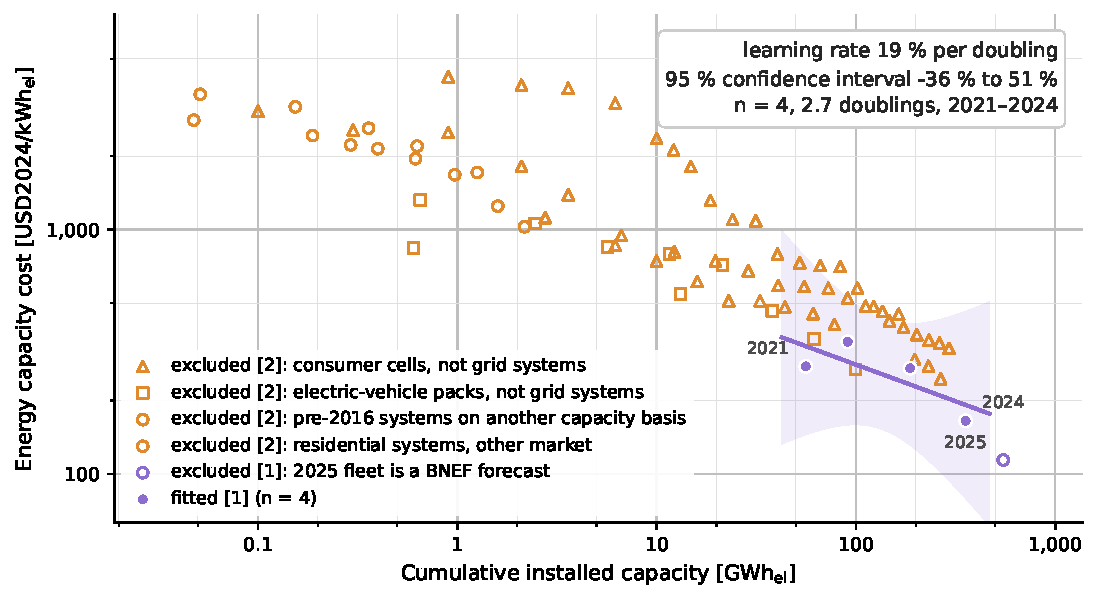
\includegraphics[width=\textwidth]{../../../misc-quarter1/technology-costs/figures/learning/battery-liion.pdf}
\caption{Li-ion energy capacity cost against cumulative capacity.
Sources: [1] turnkey system costs of the BNEF survey \citep{bnef2025}, fitted (the 2025 point is a forecast and excluded); [2] series of \citet{schmidt2018} for cells, electric-vehicle packs and residential systems, for context.
Dashed red line: the model input for the energy part.}\label{fig:liion}
\end{figure}

We set the fixed O\&M to 40~USD\textsubscript{2023}/kW/yr, because technology-data \citep{technologydata} gives it per kWh, which overprices short batteries.
The round-trip efficiency of 0.955 and the 22.5-year lifetime come from technology-data \citep{technologydata}.
Existing capacity is the 124~GW of utility-scale batteries the IEA counts at the end of 2024 \citep{iea2026}, almost all of it lithium-ion.

Sodium-ion batteries are also included under this technology.
They compete in the same role within about 20\,\% of lithium-ion cost, but perform better in the cold, so they need less temperature control in cold climates.
This nuance might be added to the model in appropriate regions.
